
\documentclass[a4paper,12pt]{article}
\usepackage[czech]{babel}
\usepackage[pdftex]{graphicx}
\usepackage[utf8]{inputenc}

\usepackage{wrapfig}
\usepackage{verbatim} 
\usepackage[unicode]{hyperref}


\setlength{\hoffset}{-1.3cm} % 1.7
\setlength{\voffset}{-2cm} % 2
\setlength{\textheight}{23.3cm}
\setlength{\textwidth}{16.4cm}


\usepackage[font=small,labelfont=bf,tableposition=top]{caption}
\DeclareCaptionLabelFormat{andtable}{#1~#2  \&  \tablename~\thetable}

\newcommand{\HRule}{\rule{\linewidth}{0.2mm}}

\let\stdsection\section
\renewcommand\section{\newpage\stdsection}

\begin{document}

% Uvodni strana

\begin{titlepage}

\begin{center}


FIT VUT v Brně, 2012\\[1.5cm]

\includegraphics[width=7cm]{./img/fit-cz.png}\\[1cm]

% Title
\HRule \\[0.4cm]
{\huge \bfseries Swarm Intelligence}\\[0.1cm]
{\LARGE Inteligence roje}
\HRule \\[0.8cm]

{\large Učební text k předmětu Inteligentní systémy (SIN)}\\[1cm]

\vfill

\end{center}

\begin{minipage}{0.4\textwidth}
\begin{flushleft} \large
\emph{Autoři textu:}\\
Bc. Tomáš \textsc{Kimer}\\
Bc. Stanislav \textsc{Heller}
\end{flushleft}
\end{minipage}

\end{titlepage}


% Obsah
\tableofcontents

% Text
\section{Úvod}
Pro tuto kapitolu se bude výborně čerpat z \cite{Blum08SwarmInt} \\
\url{http://www.springerlink.com/content/978-3-540-74089-6#section=226923&page=7&locus=23}

\begin{itemize}
  \item Obecné kecy o tom, k čemu to je, čím je to inspirováno atp.
  \item Zasazení do rámce s agenty a roboty
  \item blabla
\end{itemize}

\subsection{Biologický základ inteligence roje}
Čerpat z \cite{Blum08SwarmInt}, kapitola Biological Foundations of Swarm Intelligence
a z \cite{fleischer2005}, kapitola II/a Observations of Social Insects.
\begin{itemize}
  \item pozorování sociálního hmyzu (mravenci, včely, atp.)
  \item mechanismy pro řešení problémů
  \item feromony, vypařování
  \item komunikace a interakce mezi hmyzem (resp. agenty)
\end{itemize}


\subsection{Možnosti využití}
Kecy o tom, jak je možné swarm využít v:
\begin{itemize}
  \item telekomunikační systémy (optimalizace)
  \item robotika - výrobní, provozní a inspektční systémy, zemědělství, medicína
  \item logistika, kooperativní transport
  \item vojenství
\end{itemize}



\section{Definice základních pojmů}
\begin{itemize}
  \item Samoorganizace (\cite{fleischer2005})
  \item Emergentní jev (\cite{fleischer2005})
  \item Kolektivní inteligence (\cite{fleischer2005})
  \item Schopnost adaptace
\end{itemize}


\section{Inteligence roje v optimalizaci}
Obecné kecy o optimalizaci...

\subsection{Optimalizace mravenčí kolonií}
Pro algoritmy typu ACO bude vhodné využít \cite{Dorigo06antcolony}

\subsection{Optimalizace hejnem částic}
Tady se bude brát hlavně z \cite{Blum08SwarmOpt} a také třeba
z \cite{Blum08SwarmInt}, kapitola Swarm Intelligence in Optimization.



% -----------------------------------------------------------------------------
% SWARM ROBOTICS
% -----------------------------------------------------------------------------

\section{Hejna robotů}
Oblast, která je v odborné literatuře označována jako {\it Swarm Robotics}, byla první
disciplínou, ve které byl použit termín {\it Swarm Intelligence}. Původně bylo toto
označení určeno pro pojmenování celulárních robotických systémů \cite{BeniWang89}, v roce
1989 jej takto použil G. Beni a J. Wang. Později se termín rozšířil na souhrnný pojem
zastřešující širší škálu metod, které pomocí velkého počtu nepříliš inteligentních
a navzájem komunikujících jedinců řeší poměrně složité problémy.

\subsection{Úvod}
Podobně jako dříve uvedené přístupy, stejně tak i robotika hejna je přístupem, který
je inspirován přírodou. Sociální hmyz je známý svojí schopností koordinovat své
chování tak, aby skupina dosáhla požadovaného cíle, jehož dosažení není možné,
pokud by se o něj snažil pouze jeden jedinec. Příkladem mohou být mravenci
přenášející svoji kořist, která je několikanásobně větší, než jeden mravenec
nebo termiti, kteří staví velká termitiště z bláta, ve kterých je udržována
požadovaná teplota a úroveň vlhkosti.

\begin{figure}[here]
  \centering
  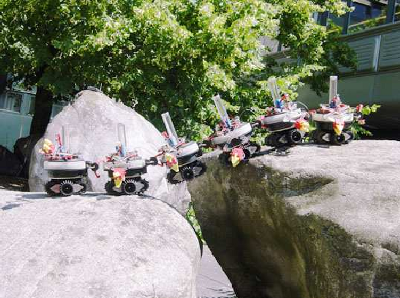
\includegraphics[width=10cm]{./img/sbot.png}
  \caption{Ukázka spolupráce robotů {\it s-bot}, kteří se snaží překonat překážku
    (propast), kterou jedinec sám překonat nedokáže.}
\end{figure}

Pro odlišení robotiky, která se zabývá hejny robotů, od ostatních směrů, které
studují multirobotické systémy, je třeba definovat, jakou oblast robotiky v sobě
zahrnuje {\it Swarm robotics}.

\paragraph{Definice.} {\it Oblast robotiky hejna se zabývá studiem
velkého počtu relativně jednoduchých, fyzicky realizovaných agentů, kteří jsou
navrženi tak, aby jejich požadované kolektivní chování bylo způsobeno pouze
lokálními interakcemi mezi agenty navzájem, případně mezi agenty a okolím.}
\cite{Sahin05}\\

Na rozdíl od nerobotického swarmu, kde jedinec v roji či hejnu byl implementován
většinou na úrovni softwarové, je zde kladen důraz na fyzickou realizaci robota
a jeho umístění do reálného prostředí. Důležitou vlastností robotů v robotickém
hejnu je schopnost fyzicky interagovat s prostředím či ostatními roboty.

Shodnou vlastností hejn robotů některými uvedenými metodami (jako např. optimalizace
mravenční kolonií) je decentralizovaná koordinace. Neexistuje zde žádný vůdce
nebo jedinec, který by direktivně řídil chování ostatních jedinců v hejnu.
Veškeré emergentní chování robotů tedy plyne pouze z lokální komunikace.

\subsubsection{Využití}
Protože je oblast robotiky hejna poměrně nová a zatím neexistují unifikované přístupy
pro návrh, implementaci a ladění robotických swarmů, není jejich komerční využití
příliš rozšířené. Mezi základní oblasti využití patří:
\begin{itemize}
  \item výrobní, provozní a inspektční systémy
  \item logistika, kooperativní transport
  \item vojenství
  \item zemědělství
  \item medicína
\end{itemize}


\subsection{Klasifikace a vlastnosti hejna robotů}
Hejno robotů můžeme klasifikovat podle různých úhlů pohledu na vlastnosti
či chování hejna \cite{Dudek93}:
\begin{description}
  \item[Velikost hejna] {- počet robotů, kteří se pohybují v daném prostředí a tvoří hejno.}
  \item[Komunikační dosah] {- ve většině systémů existují limity, které omezují
     možnosti komunikace robotů. Hlavním omezením je vzdálenost, na kterou mohou
     roboti komunikovat. Dalším faktorem může být schopnost adresace informace
     jinému robotovi, či všem robotům. Problémem může být také objem přenášených dat.}
  \item[Rekonfigurace] {- míra schopnosti hejna změnit svoji topologii. Hejno může být buď
     statické (jedna topologie) a nebo dynamické, kde vztahy mezi jedinci se může měnit.}
  \item[Výpočetní schopnost jedince] {- každý jedinec z hejna má určitou výpočetní schopnost
     odpovídající modelům, které jsou známé z teoretické informatiky. Můžeme tedy rozeznávat
     velmi jednoduché jedince, které pracují jako nelinární sumační jednotka - tyto jednotky
     pak mohou bý využity pro výstavbu a simulaci neronové sítě, ale obecně je tento model
     příliš jednoduchý, než aby se dali jedinci nazývat {\it roboty}. Dále lze uvažovat
     roboty, jejichž výpočetní model odpovídá konečnému automatu (což je preferovaným modelem
     u systémy se subsumpční architekturou). Další úrovní je zásobníkový automat, který není
     v robotice tak běžný a konečně turingův stroj, což je výpočetní model používaný dnes
     většinou robotických systémů.}
\end{description}

\subsubsection{Vlastnosti systému}
Pokud se díváme na robotické hejno jako na systém, musí splňovat tyto vlastnosti,
které u jiných multirobotických systémů splněny většinou nejsou:
\begin{itemize}
  \item {\bf Robustnost} - robotický swarm by měl být schopen pracovat i za zhoršených
    podmínek okolí - např. při rušení či při selhání některých jedinců v hejnu. Hejna
    jsou typicky redundantnm systémem - výpadek jednoho jedince může být velmi jednoduše
    a rychle nahrazen dalším. Aby bylo zamezeno častým selháním jedinců ve swarmu, měli by
    být poměrně jednoduché konstrukce na úrovni hardwarové i softwarové.
  \item {\bf Flexibilita} - hejno robotů by mělo být schopno řešit flexibilně různé úkoly.
    Inspirací v přírodě jsou mravenci, kteří díky komunikaci přes pachové stopy dokážou
    nalézt nejkratší cestu k potravě a současně jsou schopni společně velkou kořist odnést
    k mraveništi.
  \item {\bf Škálovatelnost} - použité koordinační mechanismy a strategie musí být schopny
    zajistit funkčnost swarmu při různých velikostech hejna.
  \item {\bf Homogenita} - jedinci ve swarmu by měli být homogenní, tj. buď by měli
    být identičtí z~hlediska architektury systému a schopnosti komunikace a interakce a
    nebo by měli splňovat alespoň požadavky na jednotné komunikační rozhraní a shodnost
    interakce s~okolními agenty a prostředím. Koordinační strategie, které jsou používány
    v~heterogenních multirobotických systémech, již nespadají pod přístup {\it swarm intelligence}.
\end{itemize}

\subsubsection{Požadavky na jedince}
Robotické swarmové systémy kladou na jedince (roboty) několik požadavků, které jsou
z hlediska robotiky pochopitelné, ale v oblasti obecné inteligence nejsou z důvodu
absence fyzické realizace zmiňovány. Těmito požadavky jsou:
\begin{itemize}
  \item {\bf Komunikace.} Propojení kabely a komunikace přes drátové připojení je jistě
    nedostatečné. Většina multirobotických a swarmových systémů by proto měla podporovat
    bezdrátovou komunikaci mezi roboty a také mezi konzolí a robotem pro snažší monitorování
    a ladění robotů.
  \item {\bf Fyzická interakce.} Roboti by měli umět fyzicky interagovat ve smyslu využití
    fyzických schopností svých i cizích pro dosažení určitého cíle (např. skládáním robotů
    do většího a silnějšího celku).
  \item {\bf Výdrž.} Kvůli požadavku na vysokou flexibilitu robotů ve swarmu, by mělo být
    napájení realizováno pomocí výkonných baterií. Spotřeba robotů při plnění některých
    fyzických úloh může být poměrně vysoká, proto je třeba vzít tento fakt v úvahu.
  \item {\bf Velikost robota.} V některých systémech může být kladen důraz na velikost robota.
    Ta je vždy kompromisem; miniaturizace může být v některých případech velmi nákladná,
    naopak přílišné zmenšení systému je v protikladu s případnou rozšířitelností funkcionality
    robota.
  \item {\bf Simulovatelnost.} Vývoj robotického swarmu bez použití technik modelování
    a simulace by byl velmi obtížný, ne-li nemožný. Simulace by měla být zaměřena na
    model interakcí a komunikace mezi roboty a měla by realisticky popisovat fyzické
    schopnosti robotů.
\end{itemize}

\subsubsection{Koordinační mechanismy}
V přírodě nalezneme množství koordinačních mechanismů, které byly inspirací pro robotiku.
Uveďme tedy alespoň dva hlavní principy koordinace uvnitř swarmu.
\begin{description}
  \item[Samoorganizace] {je v přírodních systémech běžná. Základním předpokladem pro
    výskyt jevů, které shrnujeme pod označení samoorganizace, je pozitivní a negativní
    odezva při lokální interakci jedinců \cite{Bonabeau99}. Dalším předpokladem je také
    existence náhody, která se v přírodě vyskytuje ve formě nepravidelností, mutací, či
    jiných jevech.}
  \item[Stigmergie] {je naopak mechanismem, který předpokládá nepřímou komunikaci
    mezi jedinci přes prostředí. Příkladem stigmergické komunikace je zanechávání feromonů
    na zemi; mravenci tímto způsobem označují cesty k potravě a tyto feromony pak pusobí
    jako atraktory.}
\end{description}

\subsubsection{Výpočetní schopnost robotického swarmu}
Robotické hejno se řadí do kategorie distribuované inteligence. Z pohledu teoretické
informatiky je jistě významné, se kterým výpočetním modelem je hejno robotů ekvivalentní.
Jistě záleží na výpočetních schopnostech jedince; avšak již u robotů, kteří jsou výpočetně
ekvivalentní konečnému automatu, lze dokázat ekvivalenci výpočetní schopnosti hejna těchto
robotů s Turingovým strojem.

Důkaz je založen na nekonečné množině komunikujících konečných automatů, u kterých jsou
rozlišeny tři druhy stavů: {\it vysílající, přijímající zleva a přijímající zprava}.
Základní myšlenkou pro simulaci turingova stroje na této množině konečných automatů je
pak předpoklad, že každý automat simuluje konečné řízení Turingova stroje a reprezentuje
jedno pole na pásce. Automat korespondující s aktuálním polem na pásce je vždy ve stavu
{\it vysílající}, automat napravo je ve stavu {\it přijímající zleva} a automat
nalevo ve stavu {\it přijímající zprava}. Přechod vysílajícího automatu pak simuluje
posun čtecí hlavy doprava, doleva či přepis symbolu na pásce. Prostudování celého důkazu
pak v případě zájmu ponecháváme již na případném čtenáři. \cite{Dudek93}


\subsection{Návrh a modelování}


\subsection{Příklady reálných systémů založených na robotice hejna}




\section{Další přístupy a metody}
\begin{itemize}
  \item cellular robotic systems, učení a adaptační strategie
  \item chaos \& swarm
\end{itemize}



\renewcommand{\refname}{\section{Použitá literatura}}
\bibliographystyle{plain}
\bibliography{refs}

\end{document}
